\documentclass{article}
\usepackage{times}
\usepackage{amsmath,amssymb}
\usepackage{tikz}
\pdfpagewidth=12.7cm
\pdfpageheight=6.8cm
\setlength{\paperwidth}{12.7cm}
\setlength{\paperheight}{6.8cm}
\setlength{\oddsidemargin}{-1in}
\setlength{\evensidemargin}{-1in}
\setlength{\topmargin}{-1in}
\setlength{\headheight}{0pt}
\setlength{\headsep}{0pt}
\setlength{\textwidth}{12.7cm}
\setlength{\textheight}{6.8cm}
\pagestyle{empty}
\tikzset{every picture/.style={line width=0.5pt}}

\begin{document}
\noindent\resizebox{\linewidth}{!}{%
\begin{tikzpicture}[x=1cm,y=1cm,baseline=(current bounding box.north)]
\node at (2.55,3.55) {\small (a) the endpoint substitution};
\draw[->] (0,0) -- (5.0,0);
\draw[->] (0,0) -- (0,3.2);
\draw (4.2,0.06) -- (4.2,-0.06) node[below] {\small $M$};
\draw (2.7,0.06) -- (2.7,-0.06) node[below] {\small $v$};
\node[below left] at (0.12,0) {\small $0$};
\draw[thick] (0,1.0) -- (4.2,2.9);
\fill (0,1.0) circle (1.6pt) node[left] {\small $G(0)$};
\fill (4.2,2.9) circle (1.6pt) node[right] {\small $G(M)$};
\draw[dash pattern=on 2pt off 2pt] (2.7,0) -- (2.7,2.22);
\fill (2.7,2.22) circle (1.6pt);
\node[above left] at (2.78,2.24) {\small $G(v)$};
\draw[|-|] (0,-0.62) -- (2.7,-0.62);
\node at (1.35,-0.95) {\small $p=v/M$};
\node[align=center] at (3.95,0.95)
  {\scriptsize one weight pins one value;\\[-1pt]\scriptsize the chord is forced};
\draw[black!30] (5.65,-1.1) -- (5.65,3.7);
\node at (9.5,3.55) {\small (b) the weight axis $p\in[0,1]$};
\draw (6.6,1.55) -- (12.4,1.55);
\draw (6.6,1.43) -- (6.6,1.67) node[below=7pt] {\small $0$};
\draw (12.4,1.43) -- (12.4,1.67) node[below=7pt] {\small $1$};
\draw[black!55] (7.244,1.55) -- (7.244,1.79);
\draw[black!55] (7.325,1.55) -- (7.325,1.79);
\draw[black!55] (7.429,1.55) -- (7.429,1.79);
\draw[black!55] (7.567,1.55) -- (7.567,1.79);
\draw[black!55] (7.760,1.55) -- (7.760,1.79);
\draw[black!55] (7.889,1.55) -- (7.889,1.79);
\draw[black!55] (8.050,1.55) -- (8.050,1.79);
\draw[black!55] (8.257,1.55) -- (8.257,1.79);
\draw[black!55] (8.533,1.55) -- (8.533,1.79);
\draw[black!55] (8.775,1.55) -- (8.775,1.79);
\draw[black!55] (8.920,1.55) -- (8.920,1.79);
\draw[black!55] (9.086,1.55) -- (9.086,1.79);
\draw[black!55] (9.178,1.55) -- (9.178,1.79);
\draw[black!55] (9.500,1.55) -- (9.500,1.79);
\draw[black!55] (9.822,1.55) -- (9.822,1.79);
\draw[black!55] (9.914,1.55) -- (9.914,1.79);
\draw[black!55] (10.080,1.55) -- (10.080,1.79);
\draw[black!55] (10.225,1.55) -- (10.225,1.79);
\draw[black!55] (10.467,1.55) -- (10.467,1.79);
\draw[black!55] (10.743,1.55) -- (10.743,1.79);
\draw[black!55] (10.950,1.55) -- (10.950,1.79);
\draw[black!55] (11.111,1.55) -- (11.111,1.79);
\draw[black!55] (11.240,1.55) -- (11.240,1.79);
\draw[black!55] (11.433,1.55) -- (11.433,1.79);
\draw[black!55] (11.571,1.55) -- (11.571,1.79);
\draw[black!55] (11.675,1.55) -- (11.675,1.79);
\draw[black!55] (11.756,1.55) -- (11.756,1.79);
\node[align=center] at (9.5,2.55)
  {\scriptsize $(J_Q)$ tests only this rational comb;\\[-1pt]
   \scriptsize a $\mathbb{Q}$-linear pathology passes every test on it};
\draw[very thick] (10.701,1.55) -- (10.701,1.06);
\fill (10.701,1.06) circle (1.5pt);
\node[align=center] at (9.5,0.45)
  {\scriptsize an irrational $p$ (here $1/\sqrt{2}$, a schematic marker): $(\star)$ tests here too,\\[-1pt]
   \scriptsize and some such test exposes any non-$\mathbb{R}$-linear defect};
\draw[->,black!60] (9.95,0.78) -- (10.62,1.0);
\end{tikzpicture}%
}%
\end{document}